\section*{Appendix}
\label{sec:appendix}

\begin{figure}[h]
    \begin{center}
        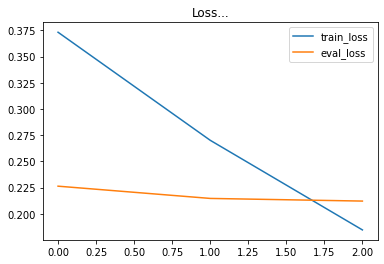
\includegraphics[width= 0.9\linewidth]{gambar/loss_concat_awal.png}
        \caption{Nilai \textit{Loss} saat Pengujian dengan Mengambil Bagian Awal Teks}
        \label{fig: loss_const_awal}
    \end{center}
\end{figure}

\begin{figure}[h]
    \begin{center}
        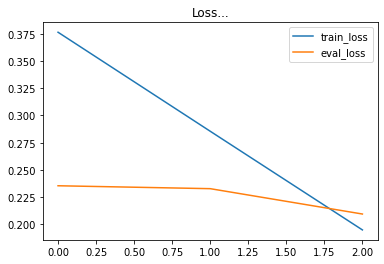
\includegraphics[width= 0.9\linewidth]{gambar/loss_concat_tengah.png}
        \caption{Nilai \textit{Loss} saat Pengujian dengan Mengambil Bagian Tengah Teks}
        \label{fig: loss_const_tengah}
    \end{center}
\end{figure}

\begin{figure}[h]
    \begin{center}
        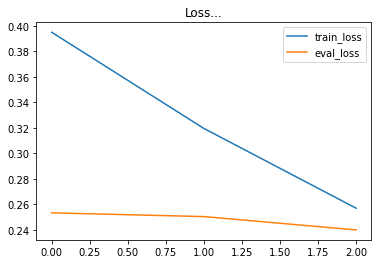
\includegraphics[width= 0.9\linewidth]{gambar/loss_bert_bahasa.png}
        \caption{Nilai \textit{Loss} saat Pengujian dengan model \textit{bert-bahasa}}
        \label{fig: loss_bert_bahasa}
    \end{center}
\end{figure}

\begin{figure}[h]
    \begin{center}
        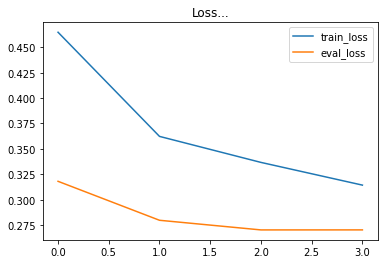
\includegraphics[width= 0.9\linewidth]{gambar/loss_bert_multilingual.png}
        \caption{Nilai \textit{Loss} saat Pengujian dengan model \textit{bert-base}}
        \label{fig: loss_bert_multilingual}
    \end{center}
\end{figure}

\begin{figure}[h]
    \begin{center}
        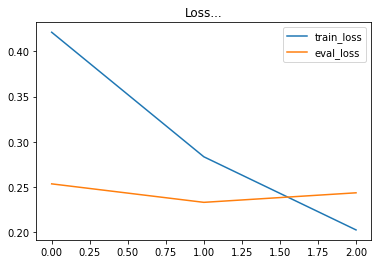
\includegraphics[width= 0.9\linewidth]{gambar/loss_cahya_bert_522.png}
        \caption{Nilai \textit{Loss} saat Pengujian dengan model \textit{cahya-522M}}
        \label{fig: loss_bert_cahya522}
    \end{center}
\end{figure}

\begin{figure}[h]
    \begin{center}
        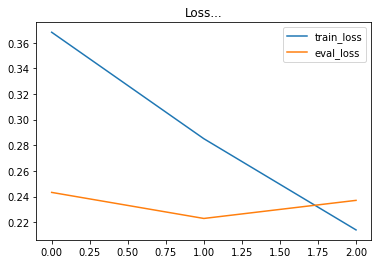
\includegraphics[width= 0.9\linewidth]{gambar/loss_cahya_bert_1,5.png}
        \caption{Nilai \textit{Loss} saat Pengujian dengan model \textit{cahya-1.5G}}
        \label{fig: loss_cahya1.5}
    \end{center}
\end{figure}

\begin{figure}[h]
    \begin{center}
        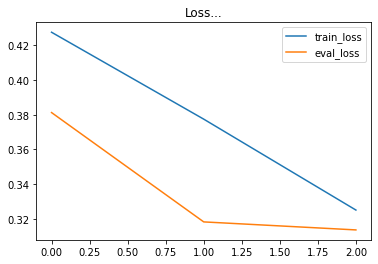
\includegraphics[width= 0.9\linewidth]{gambar/loss_roberta522.png}
        \caption{Nilai \textit{Loss} pada model ROBERTA}
        \label{fig: loss_roberta}
    \end{center}
\end{figure}


\begin{figure}[h]
    \begin{center}
        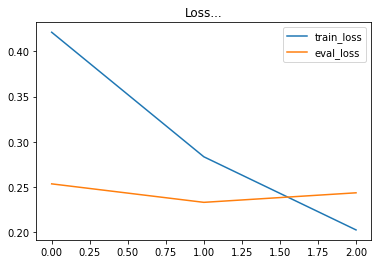
\includegraphics[width= 0.9\linewidth]{gambar/loss_cahya_bert_522.png}
        \caption{Nilai \textit{Loss} pada model BERT}
        \label{fig: loss_bert}
    \end{center}
\end{figure}

\begin{figure}[h]
    \begin{center}
        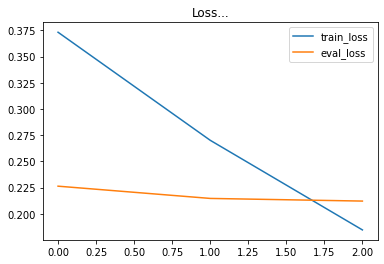
\includegraphics[width= 0.9\linewidth]{gambar/loss_concat_awal.png}
        \caption{Nilai \textit{Loss} saat Pengujian dengan model \textit{indobert}}
        \label{fig: loss_bert_indobert}
    \end{center}
\end{figure}